\documentclass{beamer}

\usetheme{Antibes}
%\usetheme{split}
% this is a template for slides using beamer package
% adapted from slides written by Ramon Medrado
% first version: Ana Bazzan
\usecolortheme[RGB={120,0,0}]{structure}
\setbeamertemplate{blocks}[rounded][shadow=true]
%\usepackage[utf8]{inputenc}   % pacote para acentuao
\usepackage[latin1]{inputenc}
\usepackage{graphicx}
\usepackage{subfigure}
\usepackage{cite}

\begin{document}
\title{Rapidly-Exploring Random Trees (RRT)}
\section{Introduction}
\frame{\frametitle{Rapidly-Exploring Random Trees (RRT)}
\begin{figure}[ht]
	\centering	
	\subfigure[ref1][Technical Report 98-11 Oct. 1998]{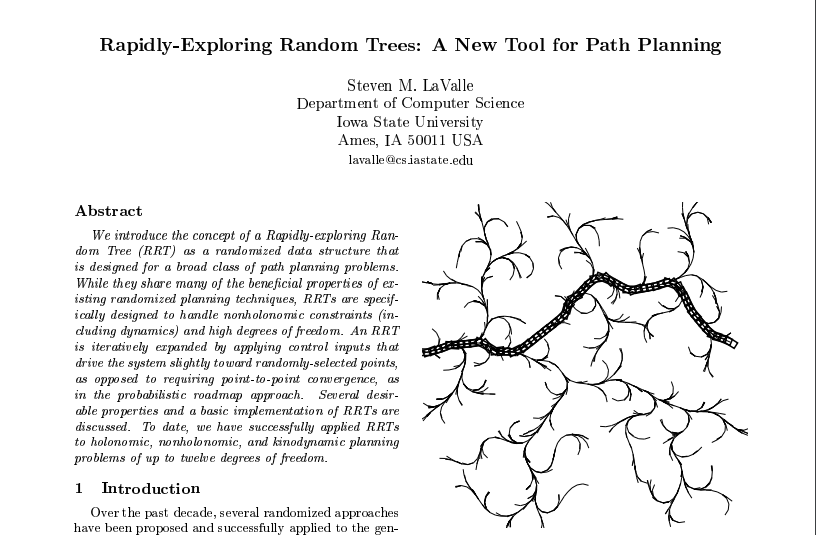
\includegraphics[scale=0.20]{artigo}}
	\subfigure[ref2][S. M. LaValle]{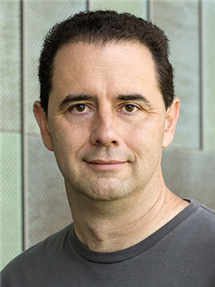
\includegraphics[scale=0.25, width=70]{lavalle}}
	\caption{Currently Professor at University of Illinois and Chief Scientist of VR/AR/MR at Huawei.}
\end{figure}
}

\section{Algorithm}
\frame{\frametitle{RRT Construction Algorithm}
\begin{figure}[ht]
	\centering	
	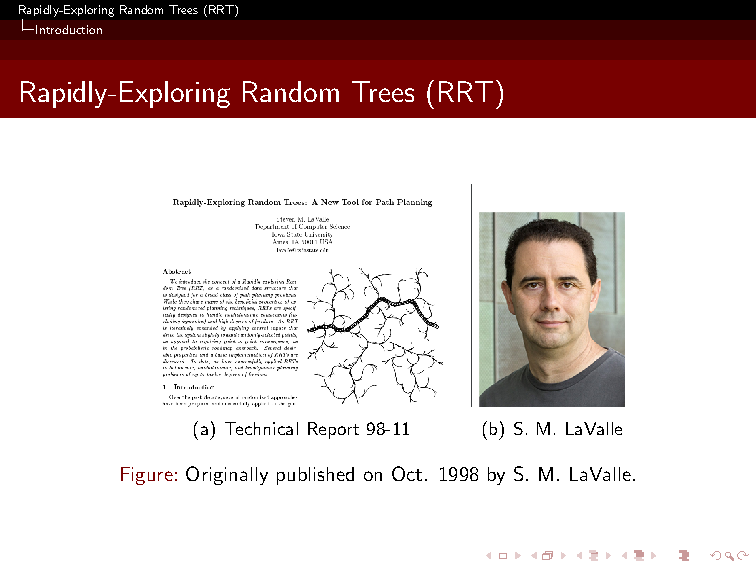
\includegraphics[scale=0.50]{rrt}
	\caption{Source [LaValle, 1998]}
\end{figure}
}

\section{Algorithm}
\frame{\frametitle{Properties}
	\begin{itemize}
	\item Relative simplicity;
	\item Bias toward unexplored space:
	\begin{itemize}
		\item State selection related to Voronoi region size;
	\end{itemize}
	\item Probabilistic completeness;
	\begin{itemize}
		\item Usually insuficient, randomness leads to zigzags.				
	\end{itemize}
	\item Input selection:
		\begin{itemize}
		\item Movement constraints;
		\item Metric effects on performance.
		\end{itemize}	
	\end{itemize}	
	\begin{figure}[ht]
		\centering	
		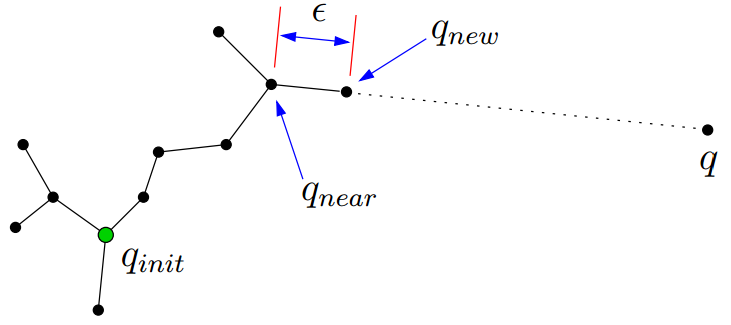
\includegraphics[scale=0.20]{example}
		\caption{Source [Kuffner \& LaValle, 2000]}
	\end{figure}
}

\section{Algorithm}
\frame{\frametitle{Variants}
	\begin{itemize}
		\item Nonholonomic constraints on tree growth:
		\begin{itemize}
			\item Articulated-body;
			\item Rigid-body.
			\item Steering;
		\end{itemize}	
		\item Obstacles:
		\begin{itemize}
			\item Selection of random free states;
			\item Transition validity for new states.
		\end{itemize}
		\item Bias toward goal:
		\begin{itemize}
			\item Avoids "bad luck";
			\item Needs to be slight.
		\end{itemize}
		\item BiRRT, RRT*, DO-RRT, BI$^2$RRT*, I-RRT-C ...	
	\end{itemize}
}

\section{References}
\frame{
\frametitle{References}
\bibliographystyle{IEEEtran}
\bibliography{rrt}
}

\end{document}




